% Desenvolvido por André Leite - DE - UFPE
% Ajustes Raydonal Ospina - DE - UFPE/UFBA

\documentclass[a4paper,12pt,oneside,onecolumn]{Config/milktest}

%---------------------- customização ----------------------

\input{Config/pacotes.tex}
\input{Config/custom.tex} 

%%%%%%%%%%%%%----- Header------%%%%%%%%%%%%%%%%%%%
\newsavebox{\mygraphic}
\sbox{\mygraphic}{
\includegraphics[scale=1.2]{Figuras/ufba.eps}}

\fancypagestyle{milktablestyle}{
    \fancyhead{}
    \fancyfoot[C]{\thepage/\pageref{LastPage}} %
}

\pagestyle{fancy}
\fancyhead{}

\fancyhead[C]{
	    \vspace{3cm}
\rput(0,2){
  \begin{minipage}{1.75cm}\centering
    
\includegraphics[width=1.75cm]{Figuras/ufbaBlack.eps}
  \end{minipage}~\hfill~\begin{minipage}{10cm}\large\centering
    \color{cor}{\scshape universidade federal da bahia}\\
    {\scshape instituto de matemática e estatística}\\
    {\scshape \medskip Programa de Pós-graduação em Estatística e Ciência de Dados}\\[10pt]
    % Aqui as informações da prova e a data
    {\normalsize\scshape  prova escrita - processo seletivo - mestrado\\ { 16/05/2024}} 
  \end{minipage}~\hfill~\begin{minipage}{1.75cm}\centering
    
\includegraphics[width=2.0cm]{Figuras/ufba.eps}
  \end{minipage}
  }}
 \fancyfoot[C]{\thepage/\pageref{LastPage}} % 

%%%%%%%%%%%%%----- Header------%%%%%%%%%%%%%%%%%%%

\usepackage{pdfpages}

\begin{document}


%------------------------------------------------
\beb
{
\begin{description}
\item[Inscrição No:] \rule{6cm}{0.4pt}
% \item[E-mail:] remail do professor
% \item[Site do curso:] \url{ urle do curso}
\item[Regras:] A prova escrita é de carater eliminatório e versa sobre Probabilidade, Inferência, e Ciência de Dados.  A prova não deve conter identificação nominal, devendo constar apenas o número de
inscrição do candidato. A prova terá a duração máxima de 4 (quatro) horas, sem direito a
consultas. A prova deve ser claramente resolvida. Seja claro e organizado. Pode fazer uso da calculadora. É expressamente {\bf proibido} o uso do celular durante a prova.
\end{description}
}
\eeb

%%%%%%%%%%%%%%%%%%%%%%%%%%%%%%%%%%%%%%%%%%%%%%%%%%%%%%%%%%%%%%%%%
\balance
%%%%%%%%%%%%%%%%%%%%%%%%%%%%%%%%%%%%%%%%%%%%%%%%%%%%%%%%%%%%%%%%%


\section*{Probabilidade}




\question \ Sejam $A$ e $B$ eventos definidos no mesmo espaço de probabilidade tais que $P(A) = 0,5$, $P(B) = 0,3$ e $P(A \cap  B ) = 0,1.$  Encontre $P(A| B^\complement),$ em que $B^\complement$ é o evento complementar de $B$.


\bigskip

\question \ Considere uma variável aleatória discreta \( X \) que pode assumir os valores 1, 2 e 3 com as seguintes probabilidades: \( P(X = 1) = 0.2 \),  \( P(X = 2) = 0.5 \) e  \( P(X = 3) = 0.3 \). Determine o valor esperado $\mu=\text{E}(X).$ 

\bigskip

 \question \ Para uma variável aleatória com distribuição normal $X\sim N(0,1)$, encontre a probabilidade $P(| X - \mu | \geqslant 1),$ em que $\mu = \text{E}(X).$
 \bigskip 

% \question \ Seja $X$ uma variável aleatória discreta que assume valores sobre o conjunto finito dos inteiros ${\cal M}=\{-n,-(n-1), \ldots, -2,-1, 0, 1, 2, \ldots, (n-1), n \}.$ A função de probabilidade da variável aleatória $X$ é definida por 
% $$
% P(X=x) = \begin{cases}
%           \frac{1}{2n+1} & \text{se} \quad x \in {\cal M}, \\
%           0 & \text{caso contrário}.
%          \end{cases}
% $$
% Determine o valor esperado $\mu=\text{E}(X).$ 
% \bigskip

% \question \ Para uma variável aleatória com distribuição normal $X\sim N(\mu,1)$, encontre a probabilidade $P(| X - \mu | \leqslant 1)$
% \bigskip 

% \question \ Em uma família com duas crianças, considere os eventos: $A=\{\text{a primeira criança é uma menina}\}$ e $B=\{\text{as duas crianças são meninas}\}$. São $A$ e $B$ eventos independentes?
% \bigskip

\section*{Inferência}

\question \ Em um estudo sobre os efeitos da doença de Alzheimer em estágio inicial na memória não declarativa, Reber et al. usaram o Teste de Fluência Verbal para estabelecer a linha de base das habilidades de linguagem e de memória semântica em idosos. Em uma amostra aleatória simples com oitenta e oito idosos, obteve-se um escore médio de 8,82 e uma variância de 7,87. Suponha que os dados são provenientes de uma população normalmente distribuída de indivíduos semelhantes com doença de Alzheimer em estágio inicial. 
Com base nestas informações, calcule:

% Preencha as sentenças com os resultados correspondentes:

\begin{itemize}[leftmargin=15.5mm]
\item[A)] O desvio-padrão do escore da amostra.
% é de ....... 2,81

% \item[B)] O erro-padrão estimado da média da amostra é de ....0,30

\item[B)] O valor para o limite inferior do intervalo de 95$\%$ de confiança (IC) para a média populacional do escore. 
% é igual a ....8,23

\item[C)] A margem de erro para um IC de 99$\%$ para a média populacional do escore.
% é de .... 0,77
\end{itemize}

\bigskip

\question \ Ao conduzir um teste de hipóteses para proporção em um estudo sobre comportamento alimentar compulsivo, se o $p$-valor for igual a 0,09, podemos rejeitar a hipótese nula de que a proporção de participantes com comportamentos alimentares compulsivos é menor ou igual a 30\%? Justifique sua resposta.

\bigskip

% \question \ Seja $X$ uma variável aleatória seguindo a distribuição de Poisson $$    f(x;\theta)=\frac{e^{-\theta} \theta^x}{x!},\,\!  \text{para} \ x=0,1,\ldots.$$ Suponha que o parâmetro $\theta$ pode assumir algum dos seguintes 3 valores,  $\theta=  4;  4,5;  5,0.$ 
% Baseado no princípio de máxima verossimilhança determine qual é o valor de $\theta$ que maximiza a probabilidade de ocorrência de uma amostra de tamanho 2 que assume os valores $x_1=2$ e $x_2=7.$
% \bigskip 

\question \  O viés de um estimador $T$ é definido como  %Ele é a distância entre a média do conjunto de estimativas, e o único parâmetro a ser estimado. 
Seja $X$ uma variável aleatória seguindo a distribuição de Bernoulli 
$$
f(x;\theta) = \theta^x(1-\theta)^{1-x} \quad \text{para} \quad {x \in \{0,1\}},  \quad  0< \theta<1.
$$
Baseado em uma amostra de tamanho $n=1$ da população de $X$ definimos os seguintes estimadores de $\theta$ como: $T_1(X)=X$ e $T_2(X)=\frac{1}{2}.$  Avalie estatisticamente se $T_1(X)$ e $T_2(X)$ são estimadores não viesados. 

\bigskip








% \question \ Se está conduzindo uma pesquisa sobre uso de mídia social em adolescentes. Seis adolescentes relatam as idades em que começaram a usar as mídias sociais: 12, 13, 14, 11, 15, 12, 11. Qual a moda dessas idades?

% \question \ Considere uma amostra aleatória de 16 estudantes, aos quais foi perguntado o número de filmes assistidos durante uma semana. Os resultados da pesquisa estão apresentados na Tabela~\ref{tab:ex1amostra}.

% \begin{table}[!htb]
% 	\begin{center}\small\sffamily
% 		\begin{tabular}{c|c|c|c} \hline
% 			No. de filmes  &  $f$ & $f_{\text{rel}}$ & $F_{\text{rel}}$\\
% \hline
% 			$0$ & $5$ & &\\		    
% 			$1$ & $5$ & &\\		    
% 			$2$ & $6$ & &\\
    
% \hline
% 		\end{tabular}
% 		\caption{Resultado da pesquisa.}
% 		\label{tab:ex1amostra}
% 	\end{center}
% \end{table}
% Note-se que na Tabela~\ref{tab:ex1amostra}  denota-se por $f$  a frequência, por $f_{\text{rel}}$ a frequência relativa e $F_{\text{rel}}$ a frequência relativa acumulada. Complete as colunas da Tabela  e encontre a média e mediana.
% \bigskip

% \question \ Ao conduzir um teste de hipóteses para proporção em um estudo sobre comportamento alimentar compulsivo, se o valor $p$-valor for 0,10, podemos rejeitar a hipótese nula de que a proporção de participantes com comportamentos alimentares compulsivos é menor que 30\%.

\section*{Ciência de Dados}


\question \  Em um sistema de detecção de spam, um modelo de classificação binária foi treinado para prever se um email é spam ou não. De 200 emails testados, 160 foram corretamente classificados. Qual é a acurácia do modelo?


\bigskip


\question \ Um modelo preditivo bastante útil em ciência de dados é o modelo de regressão linear simples onde, por exemplo,  a previsão do preço de venda de casas usa como variável independente apenas a área (em metros quadrados) da casa. Se o intercepto é 100.000 e a inclinação é 2.000 em um modelo de regressão linear simples, qual é o preço estimado de uma casa de 150 metros quadrados?


% \question \ O que é aprendizado 
% supervisionado?
% \begin{itemize}[leftmargin=15.5mm]
%     \item[A)] Uma técnica que não requer dados etiquetados.
%     \item[B)] Uma técnica que utiliza dados não etiquetados para descobrir padrões.
%     \item[C)] Uma técnica que utiliza dados etiquetados para treinar modelos.
%     \item[D)] Uma técnica exclusiva para análise de texto.
% \end{itemize}


% \question \  Um modelo de regressão linear foi utilizado para prever o preço de venda de casas com base em suas áreas (em metros quadrados). Os valores preditos e os valores reais (em miles de reais) para 5 casas foram respectivamente: (200, 210), (300, 290), (250, 260), (350, 340), (400, 410). Qual é o erro quadrático médio do modelo?
% \bigskip


% \question \ Qual das seguintes afirmações melhor descreve o termo ``Big Data''?

% \begin{itemize}[leftmargin=15.5mm]
%    \item[A)]   Dados que são coletados de uma única fonte.
%     \item[B)]  Dados que são pequenos em volume mas complexos para analisar.
%    \item[C)]  Grandes volumes de dados que são processados e analisados para revelar padrões, tendências e associações.
%    \item[D)]  Dados que não são úteis para a inteligência de negócios.
% \end{itemize}

% \vfill\eject

 \newpage
\section*{Fórmulas}

% \noindent $\bullet$ Uma variável aleatória $Z$ tem distribuição normal padrão, denotado por $Z \sim N(0,1)$  se sua função de densidade é
% $$f_Z(z)  = \dfrac{1}{\sqrt{2\pi }} e ^{-\frac{z^{2}}{2}}, \quad z\in \mathbb{R}.$$ Para esta distribuição, temos que $P(Z<2)=0,9772;$ $P(Z<1)=0,8413;$ $P(Z<-1)=0.1587$
% \bigskip

\noindent $\bullet$ A matriz de confusão dada na Tabela \ref{tab:confusion_matrix} é uma ferramenta para avaliar o desempenho de um algoritmo de aprendizado supervisionado de classificação binário. 

\begin{table}[htb]
\centering
\caption{Matriz de Confusão para um Classificador Binário}
\label{tab:confusion_matrix}
\begin{tabular}{c|c|c|}
\cline{2-3}
& \multicolumn{1}{c|}{\textbf{Previsão Positivo}} & \textbf{Previsão Negativo} \\ \hline
\multicolumn{1}{|c|}{\textbf{Real Positivo}} & Verdadeiro Positivo ($VP$) & Falso Negativo ($FN$) \\ \hline
\multicolumn{1}{|c|}{\textbf{Real Negativo}} & Falso Positivo ($FP$) & Verdadeiro Negativo ($VN$) \\ \hline
\end{tabular}
\end{table}
%em que 
%\begin{itemize}
%\item Verdadeiro Positivo (VP): O número de casos positivos corretamente identificados pelo modelo.
%\item Falso Positivo (FP): O número de casos negativos incorretamente identificados como positivos pelo modelo.
%\item Falso Negativo (FN): O número de casos positivos incorretamente identificados como negativos pelo modelo.
%\item Verdadeiro Negativo (VN): O número de casos negativos corretamente identificados pelo modelo.
%\end{itemize} 


Com base na matriz de confusão, várias métricas de desempenho podem ser calculadas:
\begin{itemize}
\item Acurácia: Proporção de todas as previsões corretas (positivas e negativas).
   \[
   \text{Acurácia} = \frac{VP + VN}{VP + VN + FP + FN}
   \]

\item Precisão: Proporção de previsões positivas que são realmente positivas.
   \[
   \text{Precisão} = \frac{VP}{VP + FP}
   \]

% \item Recall (Sensibilidade ou Taxa de Verdadeiro Positivo): Proporção de casos positivos reais que foram corretamente identificados.
%    \[
%    \text{Recall} = \frac{VP}{VP + FN}
%    \]

% \item Especificidade (Taxa de Verdadeiro Negativo): Proporção de casos negativos reais que foram corretamente identificados.
%    \[
%    \text{Especificidade} = \frac{VN}{VN + FP}
%    \]

% \item F1-Score: Média harmônica de precisão e recall.
%    \[
%    \text{F1-Score} = 2 \times \frac{\text{Precisão} \times \text{Recall}}{\text{Precisão} + \text{Recall}}
%    \]
\end{itemize}

\noindent $\bullet$ O Erro Quadrático Médio (EQM) é uma medida para avaliar o desempenho de um modelo de regressão, que é definido por
%Ele quantifica quão próximo as previsões do modelo estão dos valores verdadeiros em que sua formula é 
\[
\text{EQM} = \frac{1}{n} \sum_{i=1}^n (y_i - \hat{y}_i)^2
\] em que \( n \) é o número total de observações, \( y_i \) é o valor real da \( i \)-ésima observação e \( \hat{y}_i \) é o valor predito pelo modelo para a \( i \)-ésima observação.

\newpage
\thispagestyle{plain}
\centering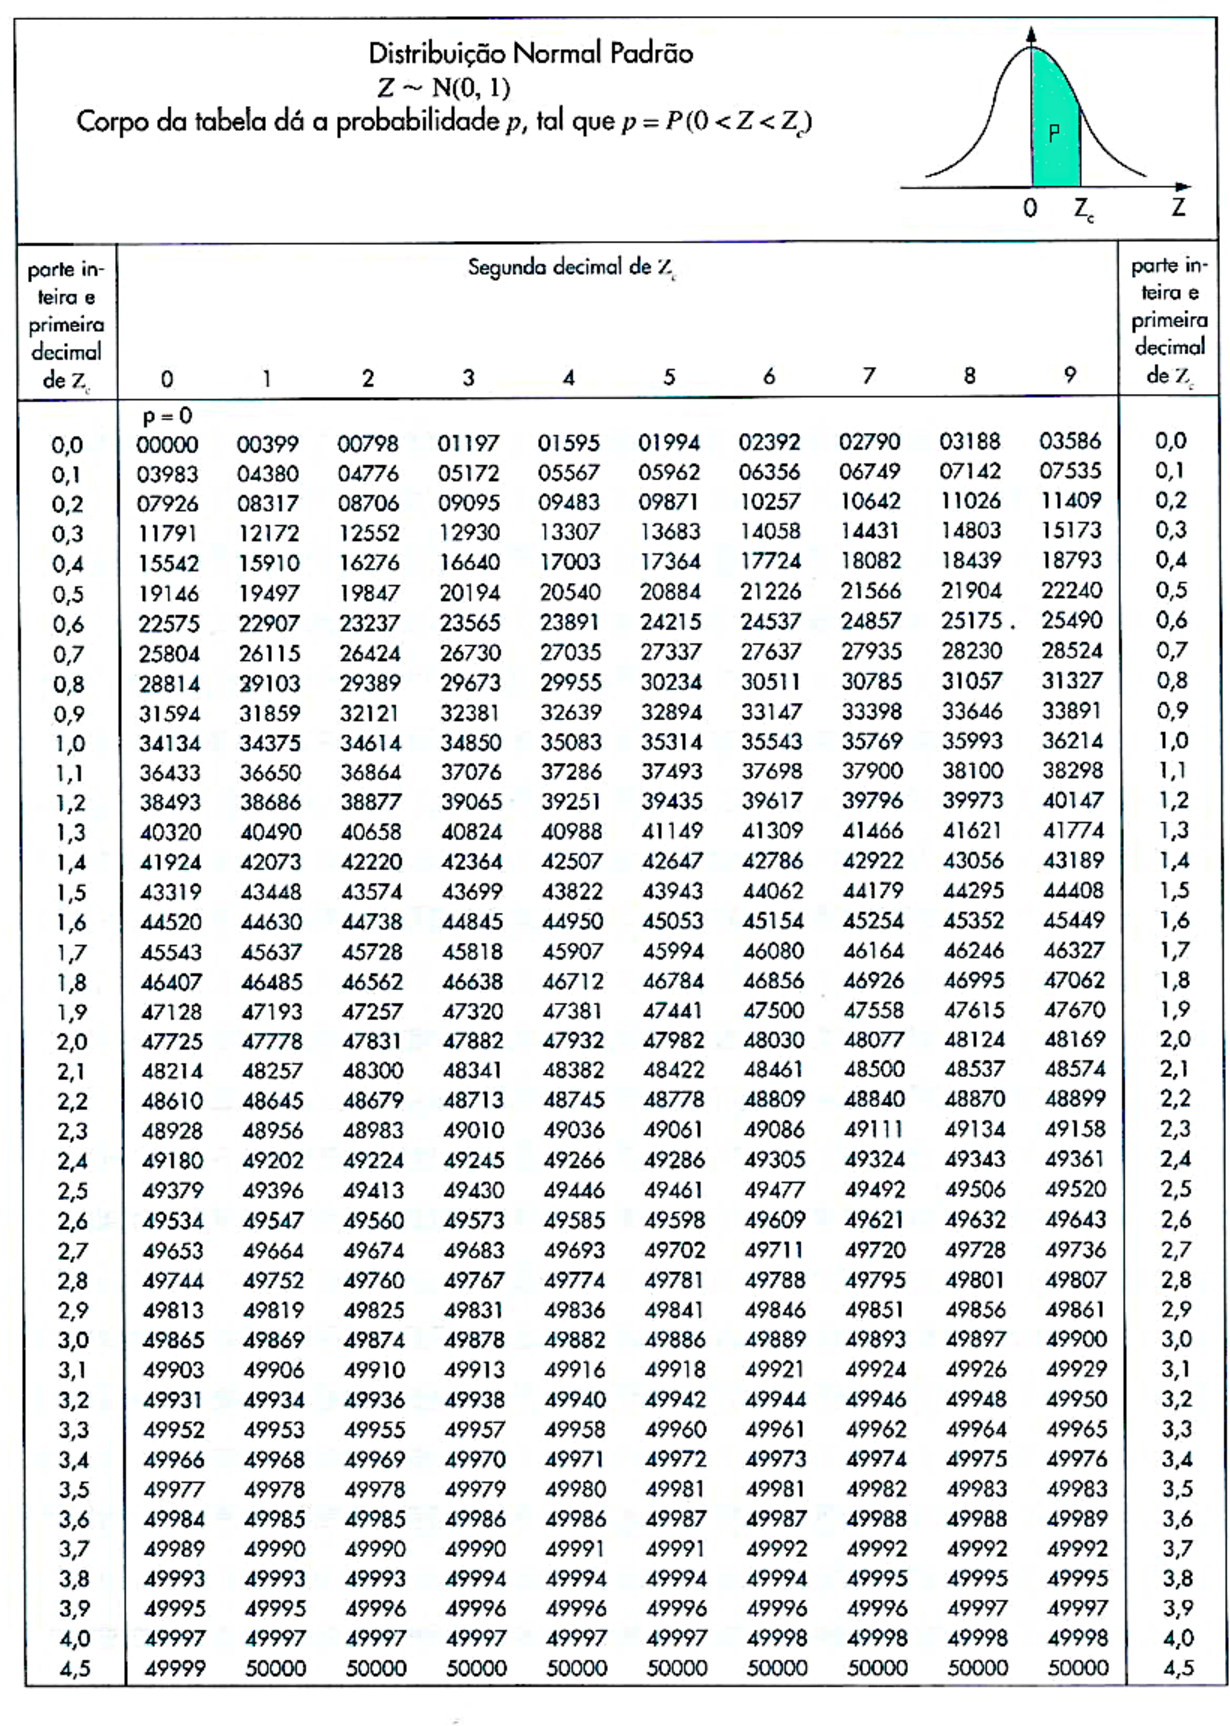
\includegraphics[scale=0.7]{Figuras/Tabela_Normal_padrao.pdf}

\end{document}

% Prova
